\apendice{Documentación técnica de programación}

\section{Introducción}
En este apéndice van a describirse de forma detallada la documentación técnica de programación. Se describirá la estructura de directorios que posee, la instalación y ejecución, así como las pruebas que se han llevado a cabo. 

El repositorio del proyecto puede ser consultado en el siguiente enlace: \textbf~\url{https://github.com/mtc1003/TF_Keras_TFG}

\section{Estructura de directorios}
\begin{itemize}
    \tightlist
    \item \texttt{/}: es la raíz del proyecto dónde se encuentran tanto el README, la licencia y las carpetas contenedoras del código, documentación y las pruebas previas.
    \item \texttt{/codigo}: es la carpeta que contiene todo el código funcional del proyecto.
    \item \texttt{/codigo/checkpoints}: es la carpeta contenedora de los modelos de detección en formato Tensorflow, Tensorflow Lite y Tensor-RT.
    \item \texttt{/codigo/checkpoints/custom-416}: carpeta que contiene el modelo de detección de las matrículas, que posee el tamaño 416.
    \item \texttt{/codigo/checkpoints/custom-416/saved\_model.pb}: modelo en formato Tensorflow(.pb) de las matrículas.
    \item \texttt{/codigo/checkpoints/heads-416}: carpeta con el modelo de las cabezas en formato Tensorflow.
    \item \texttt{/codigo/checkpoints/heads-416/keras\_metadata.pb}: punto de control del modelo de conversión a .pb.
    \item \texttt{/codigo/checkpoints/heads-416/saved\_model.pb}: modelo detector de cabezas en formato Tensorflow(.pb)
    \item \texttt{/codigo/checkpoints/yolov4-416}: carpeta con el modelo oficial de YOLOv4 en formato Tensorflow.
    \item \texttt{/codigo/checkpoints/yolov4-416/keras\_metadata.pb}: punto de control del modelo de conversión a .pb.
    \item \texttt{/codigo/checkpoints/yolov4-416/saved\_model.pb}: modelo detector de YOLOv4 en formato Tensorflow(.pb)
    \item \texttt{/codigo/checkpoints/custom\_tfl-416}: carpeta con el modelo de detección de las matrículas en formato Tensorflow previo a la conversióna TensorFlow Lite.
    \item \texttt{/codigo/checkpoints/custom\_tfl-416/saved\_model.pb}: modelo detector de matrículas en formato Tensorflow(.pb) preparado para su conversión a .tflite.
    \item \texttt{/codigo/checkpoints/custom\_tflv2-416}: carpeta con el modelo de detección de las matrículas en formato Tensorflow previo a la conversióna TensorFlow Lite.
    \item \texttt{/codigo/checkpoints/custom\_tflv2-416/saved\_model.pb}: modelo detector de matrículas en formato Tensorflow(.pb) preparado para su conversión a .tflite.
    \item \texttt{/codigo/checkpoints/custom-416-int8.tflite}: modelo de detección de las matrículas en formato TensorFlow Lite(.tflite).
    \item \texttt{/codigo/checkpoints/custom-416v2.tflite.tflite}: modelo de detección de las matrículas en formato TensorFlow Lite(.tflite)
    \item \texttt{/codigo/checkpoints/models\_trt.txt}: fichero con los enlaces de los modelos de TensorRT.
    \item \texttt{/codigo/core}: carpeta con los ficheros de configuración utilizados durante el proyecto.
    \item \texttt{/codigo/core/backbone.py}: fichero de Python que contine las funciones relacionadas con la red YOLOv4
    \item \texttt{/codigo/core/commom.py}: fichero de Python que contine la clase BatchNormalization, para los ajustes de la red YOLOv4
    \item \texttt{/codigo/core/config.py}: fichero de Python que contine permite la selección de los ficheros de etiquetas de cara al uso del modelo
    \item \texttt{/codigo/core/functions.py}: fichero de Python que contine las funciones utilizadas en a lo largo de la detección de los objetos.
    \item \texttt{/codigo/core/utils.py}: fichero de Python que contine las funciones relacionadas con la red YOLOv4.
    \item \texttt{/codigo/core/yolov4.py}: fichero de Python que retorna el modelo de YOLO correspondiente.
    \item \texttt{/codigo/data}: carpeta que contine la información necesaria para la detección.
    \item \texttt{/codigo/data/anchors}: carpeta que contiene los anchors de lass diferentes redes.
    \item \texttt{/codigo/data/anchors/basline\_anchors.txt}: fichero de anchors.
    \item \texttt{/codigo/data/anchors/basline\_tiny\_anchors.txt}: fichero de anchors tiny.
    \item \texttt{/codigo/data/anchors/yolov3\_anchors.txt}: fichero de anchors yolov3.
    \item \texttt{/codigo/data/anchors/yolov3\_anchors.txt}: fichero de anchors yolov4.
    \item \texttt{/codigo/data/classes}: carpeta que contiene los fichero de etiquetas de los diferentes modelos.
    \item \texttt{/codigo/data/classes/coco.names}: fichero con las etiquetas del modelo oficial de YOLOV4.
    \item \texttt{/codigo/data/classes/custom.names}: fichero con las etiquetas del modelo de detección de matrículas.
    \item \texttt{/codigo/data/classes/heads.names}: fichero con las etiquetas del modelo de detección de las cabezas.
    \item \texttt{/codigo/data/classes/voc.names}: fichero de etiquetas del modelo de voc.
    \item \texttt{/codigo/data/classes/yymnist.names}: fichero de etiquetas del modelo de yymnist, detector de números.
    \item \texttt{/codigo/data/dataset}: carpeta que contiene los ficheros etiquetados a la hora de evaluar un modelo (ruta de la imagen posición detectada y valor de la clase).
    \item \texttt{/codigo/data/dataset/head.txt}: fichero de evaluacion del módelo de las cabezas. 
    \item \texttt{/codigo/data/dataset/license\_plate.txt}: fichero de evaluación del modelo de las matrículas.
    \item \texttt{/codigo/data/dataset/val2017.txt}: fichero de evaluación del modelo coco.
    \item \texttt{/codigo/data/images}: carpeta que contiene diferentes imagenes para su detección.
    \item \texttt{/codigo/data/video}: carpeta que contien diferentes vídeos para su detección/contabilización.
    \item \texttt{/codigo/deep\_sort}: carpeta que contiene los diferentes ficheros en Python para su evaluacion con Object Tracking.
    \item \texttt{/codigo/deep\_sort/detection.py}: fichero Python que contiene las funciones de detección para Obejct Tracking.
    \item \texttt{/codigo/deep\_sort/iou\_matching.py}: fichero Python que tiene las funciones de la maedida iou para Object Tracking.
    \item \texttt{/codigo/deep\_sort/kalman\_filter.py}: fichero Python que contiene el algoritmo del filtro de Kalman\cite{kalman_filter}.  
    \item \texttt{/codigo/deep\_sort/linear\_assignment.py}: Fichero Python que contiene las funciones relacionadas con la asignación linear.
    \item \texttt{/codigo/deep\_sort/nn\_matching.py}: Fichero Python con funciones de ajuste del algorimto de vecinos más cercanos\cite{knn}.
    \item \texttt{/codigo/deep\_sort/preprocessing.py}: Fichero Python con las funciones del preprocesado para Object Tracking.
    \item \texttt{/codigo/deep\_sort/track.py}: fichero Python que contiene las funciones necearias para detectar los objetos y sus etiquetas correspondeitnes, con su respectivo número de identificación.
    \item \texttt{/codigo/deep\_sort/tracker.py}: fichero Python que contiene las funciones necearias para detectar los objetos y sus etiquetas correspondeitnes, con su respectivo número de identificación.
    \item \texttt{/codigo/detections}: carpeta con el lso resultados de las detecciones obtenidas mediante la línea de comandos.
    \item \texttt{/codigo/detections/images}: carpeta con el resultado de las imagenes detectadas.
    \item \texttt{/codigo/detections/videos}: carpeta con el resultado de los vídeos detectados.
    \item \texttt{/codigo/mAP}: carpeta que contiene lso resultados de la evaluaciones de los modelos, así como scripts de ayuda para ello.
    \item \texttt{/codigo/mAP/extra}: carepeta con los cripts de ayuda para la evaluación del modelo.
    \item \texttt{/codigo/mAP/extra/intersect-gt-and-pred.py}: fichero Python que calcula la intersección entre la posición real del objeto y la obtenida por el modelo, con el objetivo de evaluar la calidad del modelo.
    \item \texttt{/codigo/mAP/extra/remove\_space.py}: fichero Python que elimina lso espacios de las etiquetas de las clases de los modelos.
    \item \texttt{/codigo/mAP/ground-truth}: carpeta que contiene los ficheros .txt de cada imagen a evalaur con sus posiciones originales en formato YOLO, junto el nombre de la etiqueta que le corresponde.
    \item \texttt{/codigo/mAP/predicted}: carpeta que contiene los ficheros .txt de cada imagen a evaluar con sus posiciones detectadas en formato YOLO, junto el nombre de la etiqueta que le corresponde.
    \item \texttt{/codigo/mAP/results\_custom\_tf\_complete}: carpeta con los resultados de la evalaución del modelo de las matrículas.
    \item \texttt{/codigo/mAP/results\_heads\_tf\_complete}: carpeta con los resultados de la evalaución del modelo de las cabezas.
    \item \texttt{/codigo/mAP/main.py}: fichero Python que representa el resultado de la evalaución del modelo.
    \item \texttt{/codigo/model\_data}: carpeta que contiene el modelo mars-small128.pb, utilizado en la inicialización de Obejct Tracking.
    \item \texttt{/codigo/static}: carpeta que contiene los ficheros 'estaticos' para Flask.
    \item \texttt{/codigo/static/css}: carpeta que contiene los diferentes ficheros de estilos\cite{css} usados a lo largo de la app Flask.
    \item \texttt{/codigo/static/js}: carpeta que contiene los diferentes scripts de JavaScript\cite{js} utilizados a lo largo de la app Flask.
    \item \texttt{/codigo/static/detections}: carpeta que contiene las imagenes, videos etiquetados tras su detección, así como los ficheros CSV de las posiciones.
    \item \texttt{/codigo/static/imgs}: carpeta con todas las imagenes usadas a lo largo de la app Flask.
    \item \texttt{/codigo/temp}: carpeta que almacena los ficheros de detección temporales, generados al inicio de las detecciones en la app Flask.
    \item \texttt{/codigo/templates}: carpeta que contienelos ficheros .html usados a lo alrgo de la app Flask.
    \item \texttt{/codigo/tools}: carpeta que contiene los scripts Python utilizados cómo herramientas a la hora de detectar.
    \item \texttt{/codigo/tools/freeze\_model.py}: script Python que convierte el gráfico del modelo de TensorFlow a uno con extensión .pb.
    \item \texttt{/codigo/tools/generate\_detections.py}: script Python que obtiene las 'cajas' en las cuáles se encuentran los objetos qu ehan sido detectados por el modelo.
    \item \texttt{/codigo/train}: carpeta que tiene los scripts de Python y de GoogleColab, así como los ficheros neecsarios para llevar a cabo el entrenamiento de un modelo de YOLOv4.
    \item \texttt{/codigo/trt}: carpeta que contiene el script de GoogleColab de conversión del fichero de pesos de YOLOv4 (.weights) a un modelo de TensorRT.
    \item \texttt{/codigo/app.py}: fichero de Python que es la propia app de Flask.
    \item \texttt{/codigo/convert\_tflite.py}: fichero de Python que convierte el modelo deseado a uno de TensorFlow Lite.
    \item \texttt{/codigo/convert\_trt.py}: fichero de Python que convierte el modelo deseado a uno de TensorRT.
    \item \texttt{/codigo/detect.py}: fichero de Python que detecta objetos en una imagen, según un modelo de detección.
    \item \texttt{/codigo/detectVideo.py}: fichero de Python que detecta objetos en una vídeo, según un modelo de detección.
    \item \texttt{/codigo/evaluate.py}: fichero de Python que evalua un modelo de detección, con el objetivo de medir su calidad a l hora de predeccir.
    \item \texttt{/codigo/objectTracker.py}: fichero de Python que contabiliza objetos en un vídeo, según un modelo de detección.
    \item \texttt{/codigo/preprocessDataEvaluate.py}: fichero de Python que obtiene las posiciones de las imágenes en el formato necesario apra su evalaución.
    \item \texttt{/codigo/save\_model\_tflite.py}: fichero de Python que convierte un fichero de pesos en formato .weights a un modelo de TensorFlow Lite. 
    \item \texttt{/codigo/save\_model.py}: fichero de Python que convierte un fichero de pesos en formato .weights a un modelo de TensorFlow.  
\end{itemize}

\section{Manual del programador}
En esta subsección se describen todos los recursos utilizados para poder llevar a cabo el proyecto.
De tal forma que un futuro desarrollador/mantenedor del proyecto no tenga inconvenientes a la hora de retomar el proyecto y conocerlo.

\subsection{Entorno de desarrollo}
Para poder continuar con el desarrollo del proyecto, será necesario contar con el siguiente \textit{software} instalado en el equipo:
\begin{itemize}
    \tightlist
    \item Python 3.7
    \item Bibliotecas de Python
    \item VSCode
    
\end{itemize}

A continuación, se comentára de forma detallada la instalación de los diferentes requerimientos.

\subsection{Python 3.7}
La versión de Python 3.7, se encuentra dispnible desde \cite{pythonDownload}. Es muy importante que los ficheros binarios se encuentren en el PATH del sistema, para evitar así posibles problemas de ejecución.

\subsection{Bibliotecas de Python}
Este punto, es de los más importantes para hacer funcionar el proyecto, ya que son necesarias unas determiandas librerías y en unas versiones concretas, para que todo se integre correctamente y así funcione todo
cómo un sistema homogéneo. Ver Tabla~\ref{tab:bibliotecas-python}

\begin{table}[p]
    \centering
    \begin{tabular}{lcl}
        \toprule
        \textbf{Biblioteca} & \textbf{Versión} & \textbf{Descripción}\\
        \midrule
        \rowcolor[HTML]{EFEFEF} 
        \texttt{absl-py} & 0.15.0 & Creación de aplaicaciones sencillas.\\
        \texttt{flask} & 1.1.2 & Web \textit{framework}.\\ \rowcolor[HTML]{EFEFEF}
        \texttt{numpy} & 1.22.3 & Computación de \textit{arrays}.\\
        \texttt{pandas} & 0.25.1 & Estructuras de datos.\\ \rowcolor[HTML]{EFEFEF}
        \texttt{requests} & 2.27.0 & \textit{Requests} para humanos.\\
        \texttt{keyboard} & 0.13.5 & Interacción del teclado desde Python\\ \rowcolor[HTML]{EFEFEF}
        \texttt{pafy} & 0.5.5 & Recuperar contenido y metadatos de YouTube\\        
        \texttt{youtube-dll} & 2020.12.2 & Descargar vídeos de Youtube junto con su información\\ \rowcolor[HTML]{EFEFEF}
        \texttt{pandas} & 1.3.5 & Potentes estructuras de datos para análisis de datos, series temporales y estadísticas\\
        \texttt{numpy} & 1.21.6 & Paquete de computación matricial\\ \rowcolor[HTML]{EFEFEF}
        \texttt{opencv-python} & 4.1.1.26 & Visión Artificial para el lenguaje Python\\
        \texttt{tensorflow} & 2.8.0 & Framework dw Machine Learning\\ \rowcolor[HTML]{EFEFEF}
        \texttt{tensorflow-gpu} & 2.3.0 & Framework de Machine Learning para GPU\\
        \texttt{pillow} & 9.2.0 & Librería de imágenes\\ \rowcolor[HTML]{EFEFEF}
        \texttt{easydict} & 1.9 & Acceso a los valores de un \textit{dict} como atributos\\
        \texttt{matplotlib} & 3.5.3 & Trazado en Python\\ \rowcolor[HTML]{EFEFEF}
        \bottomrule
    \end{tabular}
    \caption{Bibliotecas utilizadas y sus versiones.}\label{tab:bibliotecas-python}
\end{table}

Las versiones que se indican en la Tabla~\ref{tab:bibliotecas-python}, son las que se han utilizado a lo largo del desarrollo del proyecto, las cuáles pueden ser actualizadas a versiones futuras, siempre y cuando estás sean compatibles entre sí o con las páginas web con las que trabajan por debajo.

\section{Compilación, instalación y ejecución del proyecto}

En esta sección, se va a detallar el proceso a seguir para poder poseer el proyecto en local, y así poder utilizarlo y/o modificarlo. 

\subsection{Adquisición del código fuente}
El primer paso, es la obtención del código en el equipo, para ello podremos seguir una de las siguientes aproximaciones:

\begin{itemize}
    \item Mediante el uso de la terminal.
    \begin{enumerate}
    \tightlist
    \item Apertura de la terminal.
    \item Desplazarse al directorio en donde se desee clonar el repositorio (usando \texttt{cd} en Unix o \texttt{dir} en Windows).
    \item Hacer uso del siguiente comando:\\
    \texttt{git clone https://github.com/mtc1003/TF\_Keras\_TFG.git}
    \item Se dispone de una copia idéntica a la alojada en el repositorio de \texttt{GitHub}.
    \end{enumerate}
    
    \item Descarga desde el navegador.
    \begin{itemize}
    \tightlist
    \item Apertura del navegador de preferencia.
    \item Introducir en la barra de búsqueda la siguiente dirección:\\
    \texttt{https://github.com/mtc1003/TF\_Keras\_TFG/archive/refs/heads/master.zip}
    \item Aceptar la descarga en caso de tener habilitada la comprobación.
    \item Navegar con el Explorador de archivos del sistema hasta el directorio de descarga.
    \end{itemize}

    \item Uso de \texttt{Fork}.
    \begin{itemize}
    \tightlist
    \item Apertura de la aplicación.
    \item Hacer \textit{click} en \textit{File} y del desplegable de opciones seleccionar \textit{Clone}.
    \item Dentro de la ventana de \textit{Clone}:
    \begin{itemize}
    \item En \textit{Respository Url} introducir:\\ https://github.com/mtc1003/TF\_Keras\_TFG.git.
    \item En \textit{Parent Folder} introducir: la ruta en la que se clonará el repositorio en local.
    \item En \textit{Name} introducir: el nombre que recibirá el proyecto en lcoal.
    \end{itemize}
    \item Hacer \textit{click} en \textit{Clone}.
    \end{itemize}
\end{itemize}

\subsection{Creación de entorno virtual de trabajo}
Para poder trabajar con este proyecto (independientemente de si es para desarrollo o producción) hacen falta una serie de bibliotecas concretas de Python (en unas versiones determinadas), las cuáles, como es lógico, deben estar en la máquina en la que se va a ejecutar, es decir, en la que se encuentra el código. 
El proyecto está preparado para crear un entorno de \texttt{Conda} propio, de forma que no interfiera con otros proyectos y sea más sencillo de mantener y actualizar.

Se recomienda que los binarios de anaconda o miniconda estén configurados en el \texttt{path} del sistema para poder utilizar el comando \texttt{conda} desde la línea de comandos.

El proceso de creación del entrono virtual con \texttt{Conda} es el siguiente:
\begin{enumerate}
\tightlist
\item Apertura de la terminal.
\item Navegar hasta la raíz del proyecto.
\item Crear el entorno con:\\
\texttt{conda env create -f OD\_MTC.yml}
\item Cuando se desee utilizar se debe activar:\\
\texttt{conda activate ODMTC}
\end{enumerate}

También se puede utilizar el procedimiento habitual para importar las bibliotecas al actual \texttt{venv} de la sesión de la terminal, pero se desaconseja su uso ya que un entorno 'genérico' antes o después se actualizará por otros proyectos, pudiendo generar incompatibilidades con el proyecto.

\section{Pruebas del sistema}
En está sección se van a describir las pruebas que se realizan con un modelo entrenado previamente, para así conocer su fiabilidad.

Lo primero será seleccionar el fichero de etiquetas con el que deseamos trabajar para evaluación, para ello se deberá de modificar la línea \textit{\_\_C.YOLO.CLASSES} del fichero \textit{config.py}, con el fichero de etiquetas con las clases del modelo a evaluar.
\imagen{pruebaEval}{Selección del fichero de etiquetas}
Tras esto deberemos de crear una carpeta con las imágenes, con las que deseamos evaluar el modelo y con los ficheros \textit{txt} de cada imagen con las posiciones de los objetos detectados

\imagen{headImgEval}{Ejemplo de imágen que se usará para evaluar el modelo}
\imagen{headPosEval}{Ejemplo de etiqueta que se usará para evaluar el modelo}

Tras esto, deberemos ejecutar el script \textit{preprocessDataEvaluate.py}, el cuál nos devolverá un único fichero con toda la información de las imágenes en formato YOLO.
\imagen{pdeHead}{Comando \textit{preprocessDataEvaluate.py} con el flag \textit{positions} con la ruta de las imágenes y el flag \textit{name\_txt\_export} con el nombre del fichero que se exportará}

El fichero que obtendremos será de este estilo:
\imagen{textHeadEval}{Fichero con todas las imágenes y sus posiciones en formato YOLO junto con la clase del objeto detectado}
En él, encontaremos el PATH a la imagen, la posición del objeto detectado (como x, y, width, height) y el valor de la etiqueta con la que se corresponde el objeto, estos dos últimos valores se repetirán tantas veces como objetos halla en la imagen. El fichero contará con tantas líneas como imagenes para evaluar tengamos en la carpeta.

Con este fichero ya podremos evalaur el modelo, para ello usaremos el script \textit{evaluate.py}
\imagen{evalHead}{Script \textit{evaluate.py} junto con los flags \textit{weights} con el modelo que se quiere evaluar y \textit{annotation\_path} con el PATH del fichero obtenido previamente}
Durante la ejecución de la evalaución obtendremos por pantalla el siguiente resultado:
Donde contaremos con las posiciones originales, dónde por cada detección veremos el nombre de la clase, así como las posiciones de la imagen, y las posiciones detectadas dónde tendremos el nombre de la clase, el \textit{accuraccy} de la detección y la psoción en la que se encuentra el objeto.
\imagen{resultEval}{Ejemplo del resultado de una imagen}

Por último, para ver el resultado, tendremos que movermos a la carpeta \textit{mAP} y ejecutar el script \textit{main.py}.
Donde podremos ver el resultado del \textit{mAP}

\begin{figure}[!h]
    \centering
    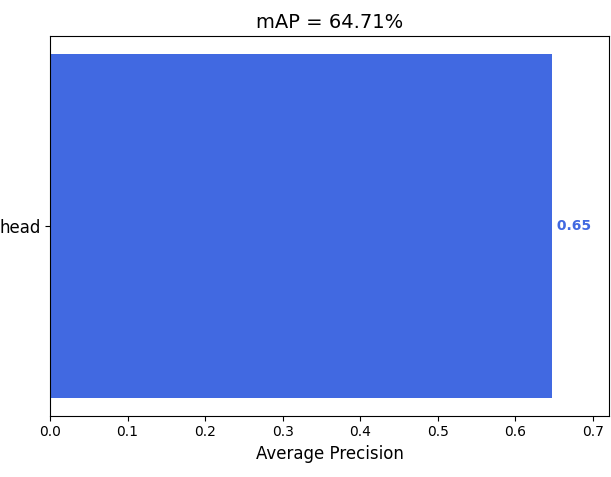
\includegraphics[width=0.6\textwidth]{evalMAP}
    \caption{mAP del modelo de detección de las cabezas}\label{fig:evalMAP}
\end{figure}

\begin{figure}[!h]
    \centering
    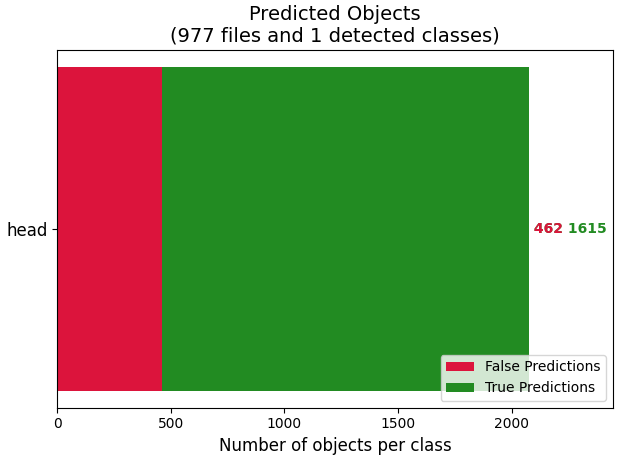
\includegraphics[width=0.6\textwidth]{infoEval}
    \caption{información sobre la evaluación del modelo}\label{fig:infoEval}
\end{figure}

\begin{figure}[!h]
    \centering
    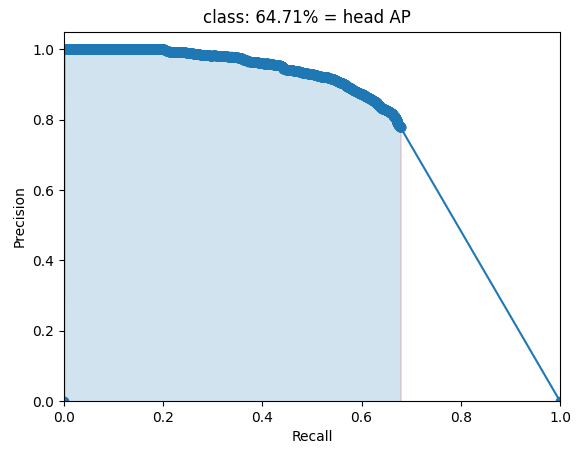
\includegraphics[width=0.6\textwidth]{prEval}
    \caption{Precission-Recall de la clase \textit{head}}\label{fig:prEval}
\end{figure}